\subsection{注意力后向传播}
\label{sec:bwd}

\subsubsection{资源分析}

与前向传播类似，我们首先通过分析屋顶线为内核设计和优化提供直觉，分析基于矩阵乘法单元（张量核心）、共享内存（smem）和指数运算单元的吞吐量。

设$\vQ$和$\vK$的序列长度维度上的块形状为$M \times N$，头维度为$d$。我们分析计算和内存流量需求以识别性能瓶颈。与前向传播不同，为简化smem周期数的公式，我们假设$M = N = d = 128$，但保留变量名以明确表达。

\noindent\textbf{MMA计算。}
后向传播每次迭代执行五次矩阵乘加（MMA）操作。每次MMA涉及一个$M \times N$矩阵、一个$M \times d$矩阵和一个$d \times N$矩阵（变化输出矩阵），需要$2MNd$次浮点操作。张量核心吞吐量为每周期8192次FLOP，总计算时间为
{\setlength{\abovedisplayskip}{2pt}%
 \setlength{\belowdisplayskip}{2pt}%
 \setlength{\abovedisplayshortskip}{2pt}%
 \setlength{\belowdisplayshortskip}{2pt}%
\begin{equation}
    T_{\text{MMA}} = \frac{10MNd}{8192} \text{ 周期。}
\end{equation}}

\noindent\textbf{共享内存流量。}
五次MMA中，三次——$\vS^\top = \vK \vQ^\top$、$\vdP^\top = \vV \vdO^\top$和$\vdQ = \vdS \vK$——是共享-共享（SS）操作，两个操作数均从共享内存读取；另外两次——$\vdV = \vP^\top \vdO$和$\vdK = \vdS^\top \vQ$——是张量-共享（TS）操作，操作数$A$从张量内存读取，操作数$B$从共享内存读取。SS MMA从共享内存合计读取$2Md + 3Nd + MN$个元素，TS MMA从共享内存合计读取$2Md$个元素。以每周期128字节的共享内存带宽和每元素2字节（bf16）计，贡献为
{\setlength{\abovedisplayskip}{4pt}%
 \setlength{\belowdisplayskip}{4pt}%
 \setlength{\abovedisplayshortskip}{3pt}%
 \setlength{\belowdisplayshortskip}{3pt}%
\begin{equation}
    T_{\text{smem,MMA}} = \frac{4 M d + 3 N d + M N}{64} \text{ 周期。}
\end{equation}}
此外，算法将大小为$M \times N$的中间梯度$\vdS$以bf16写入共享内存，需要$2MN$字节或$MN/64$周期。大小为$M \times d$的梯度$\vdQ$以fp32（每元素4字节）写入共享内存，然后通过TMA读回用于规约，共$8Md$字节的共享内存流量或$Md/16$周期。

总共享内存访问时间（$T_{\text{smem}}$）因此为
{\setlength{\abovedisplayskip}{4pt}%
 \setlength{\belowdisplayskip}{4pt}%
 \setlength{\abovedisplayshortskip}{3pt}%
 \setlength{\belowdisplayshortskip}{3pt}%
\begin{equation}
    \frac{4 M d + 3 N d + M N}{64} + \frac{MN}{64} + \frac{Md}{16} \text{ 周期。}
\end{equation}}

\begin{figure*}[t]
  \centering 
  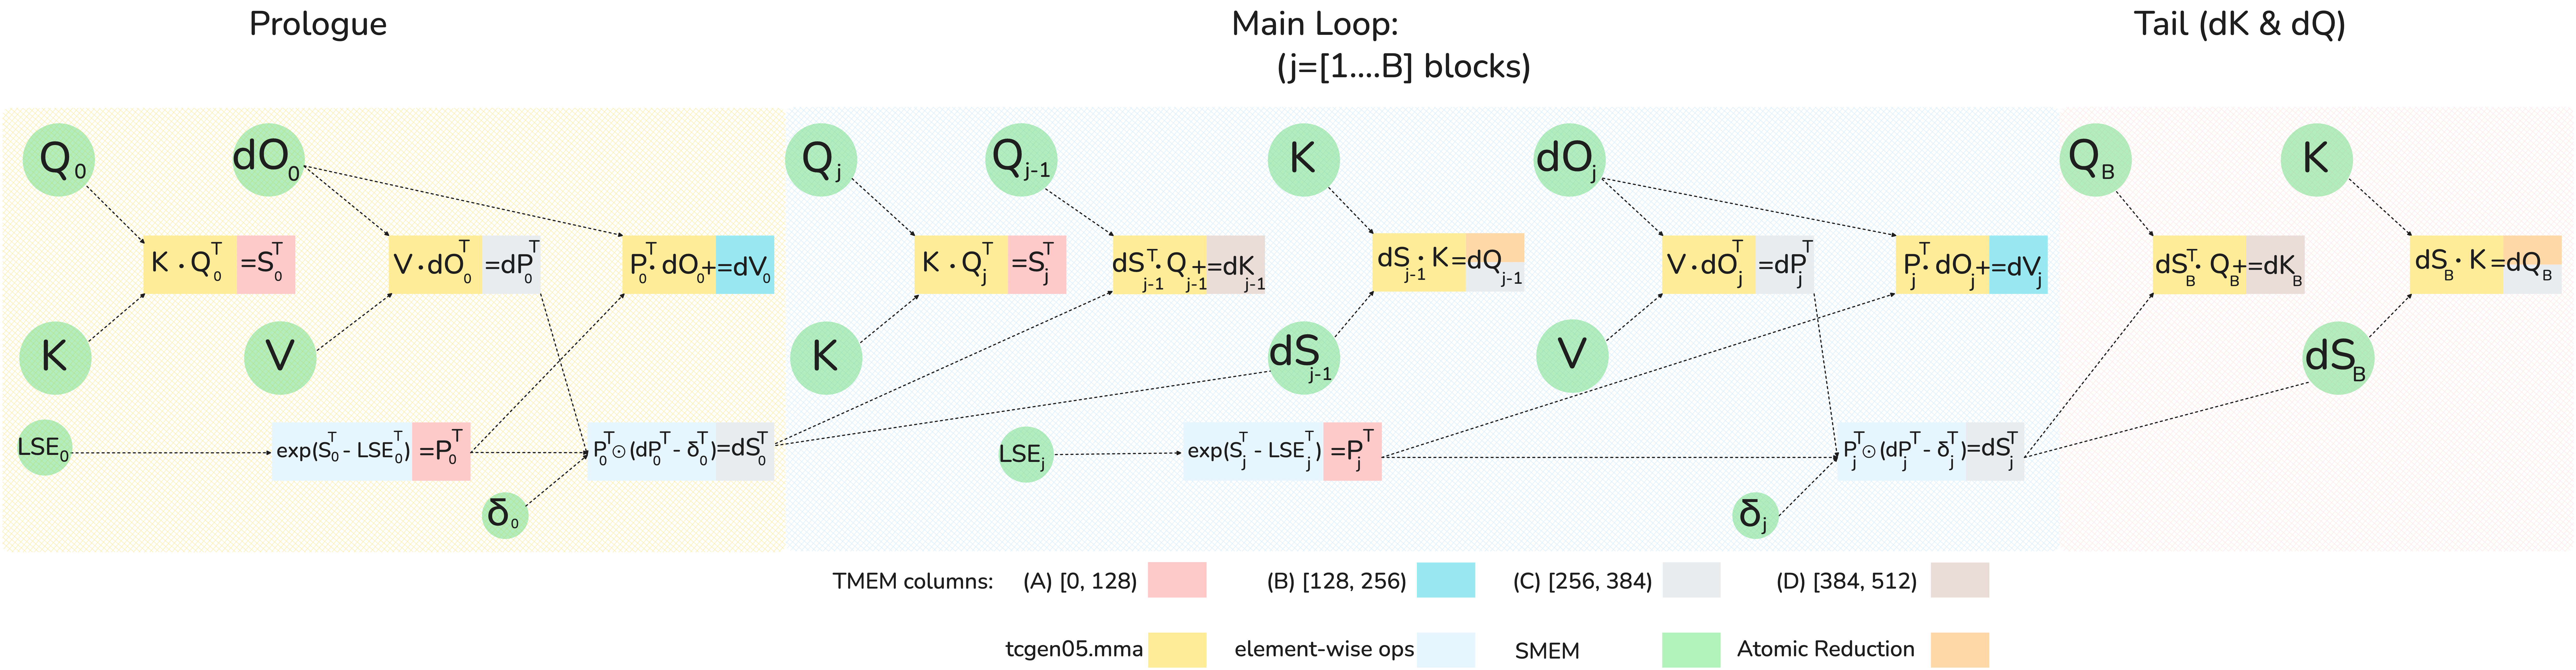
\includegraphics[width=1.0\linewidth]{Figures/fa_bwd_p8.png}
  \caption{FlashAttention-4后向传播计算图（5次MMA操作 + 2次逐元素操作），展示1-CTA MMA模式软件流水线在序言、主循环和尾声中的顺序。}
  \label{fig:bwd_computational_graph}
\end{figure*}

\noindent\textbf{指数运算单元。}
指数运算单元执行softmax及其梯度所需的逐元素操作（指数、对数及相关非线性函数）。后向传播需要对$M \times N$个值（对应注意力矩阵$\vS$及相关项）进行指数运算。吞吐量为每周期16次操作，指数运算单元所需时间为
{\setlength{\abovedisplayskip}{1pt}%
 \setlength{\belowdisplayskip}{1pt}%
 \setlength{\abovedisplayshortskip}{1pt}%
 \setlength{\belowdisplayshortskip}{1pt}%
\begin{equation}
    T_{\text{exp}} = \frac{MN}{16} \text{ 周期。}
\end{equation}}
表~\ref{tab:bwd_roofline}总结了典型分块配置$M = N = d = 128$的分析结果。共享内存流量时间3328周期超过了MMA计算时间（2560周期）和指数运算单元时间（1024周期），表明共享内存带宽是主要瓶颈，尽管程度不如全局内存流量那么严重。这为我们的内核设计提供了动力：最大化MMA操作与其他计算之间的重叠以隐藏共享内存延迟。

\begin{table}[t]
\centering
\begin{tabular}{lcc}
\toprule
资源 & 周期数（$N = d = 128$） & 周期数（$N = d = 128$） \\
         & \textbf{1-CTA}（$M = 128$） & \textbf{2-CTA}（$M = 256$） \\
\midrule
MMA计算 & 2560 & 2560 \\
共享内存（MMA操作数）& 2048 & 1536 \\
共享内存（$\vdS$写入）& 256  & 256 \\
共享内存（$\vdS$ DSMEM）& 0 & 384 \\
共享内存（$\vdQ$写入+读出）& 1024 & 512 \\
\textbf{共享内存总计} & \underline{\textbf{3328}} & \underline{\textbf{2688}} \\
指数运算单元 & 1024 & 1024\\
\bottomrule
\end{tabular}
\caption{$M = N = d = 128$时注意力后向传播的屋顶线分析。共享内存流量是瓶颈，比MMA计算时间多约30\%。在$M = 256$、$N = d = 128$的2-CTA设置中（$\vdQ$ MMA例外，其$M = N = 128$，$d = 256$），共享内存流量比MMA计算时间多约5\%。}
\label{tab:bwd_roofline}
\end{table}

\subsubsection{重叠矩阵乘法与softmax的新流水线}

FlashAttention后向传播执行五次MMA操作，对应于重新计算$\vS$，以及$\vQ \vK$（产生$\vdQ$和$\vdK$）和$\vP \vV$（产生$\vdP$和$\vdV$）诱导的两组梯度计算。
在FA-3中，累加器存储在寄存器中，寄存器是有限资源。
这施加了显著的排序约束，实际上串行化了计算图，即按顺序计算$\vS, \vdP, \vdV, \vdQ, \vdK$，只有TMA加载可以大幅乱序执行。
此外，算法类似：它沿KV序列长度维度迭代并以相对前向传播转置的方式计算值，因为$\vdV$和$\vdK$梯度计算需要从张量内存读取其一个操作数所要求的布局。
$\vdQ$通过原子操作累积。

在FA-4中，TMEM与FA-3相比实现了额外的调度方案，提供了MMA与非MMA操作之间的显著重叠。
具体地，与前向传播一样，我们试图隐藏softmax计算的延迟。
在FA-3中，softmax计算与$\vdP$的MMA重叠。
从前一节可知，在Blackwell上我们需要同时运行至少两次MMA操作。

我们通过利用前一次迭代的$\vdQ$和$\vdK$ MMA来实现这一点。
这需要在加载、MMA、计算和规约操作之间仔细管理共享内存和张量内存资源。
特别地，注意我们没有足够的张量内存来容纳五个累加器块。
最多可以容纳四个128 × 128元素的块，且$\vdV$和$\vdK$需要累积，因此不能共享它们的空间。
在我们的实现中，$\vS$和$\vP$共享一个tmem块（偏移量为0），$\vdP$、$\vdS$和$\vdQ$共享另一个。FA-4后向传播的计算图见图~\ref{fig:bwd_computational_graph}。

\begin{figure*}[t]
  \centering 
  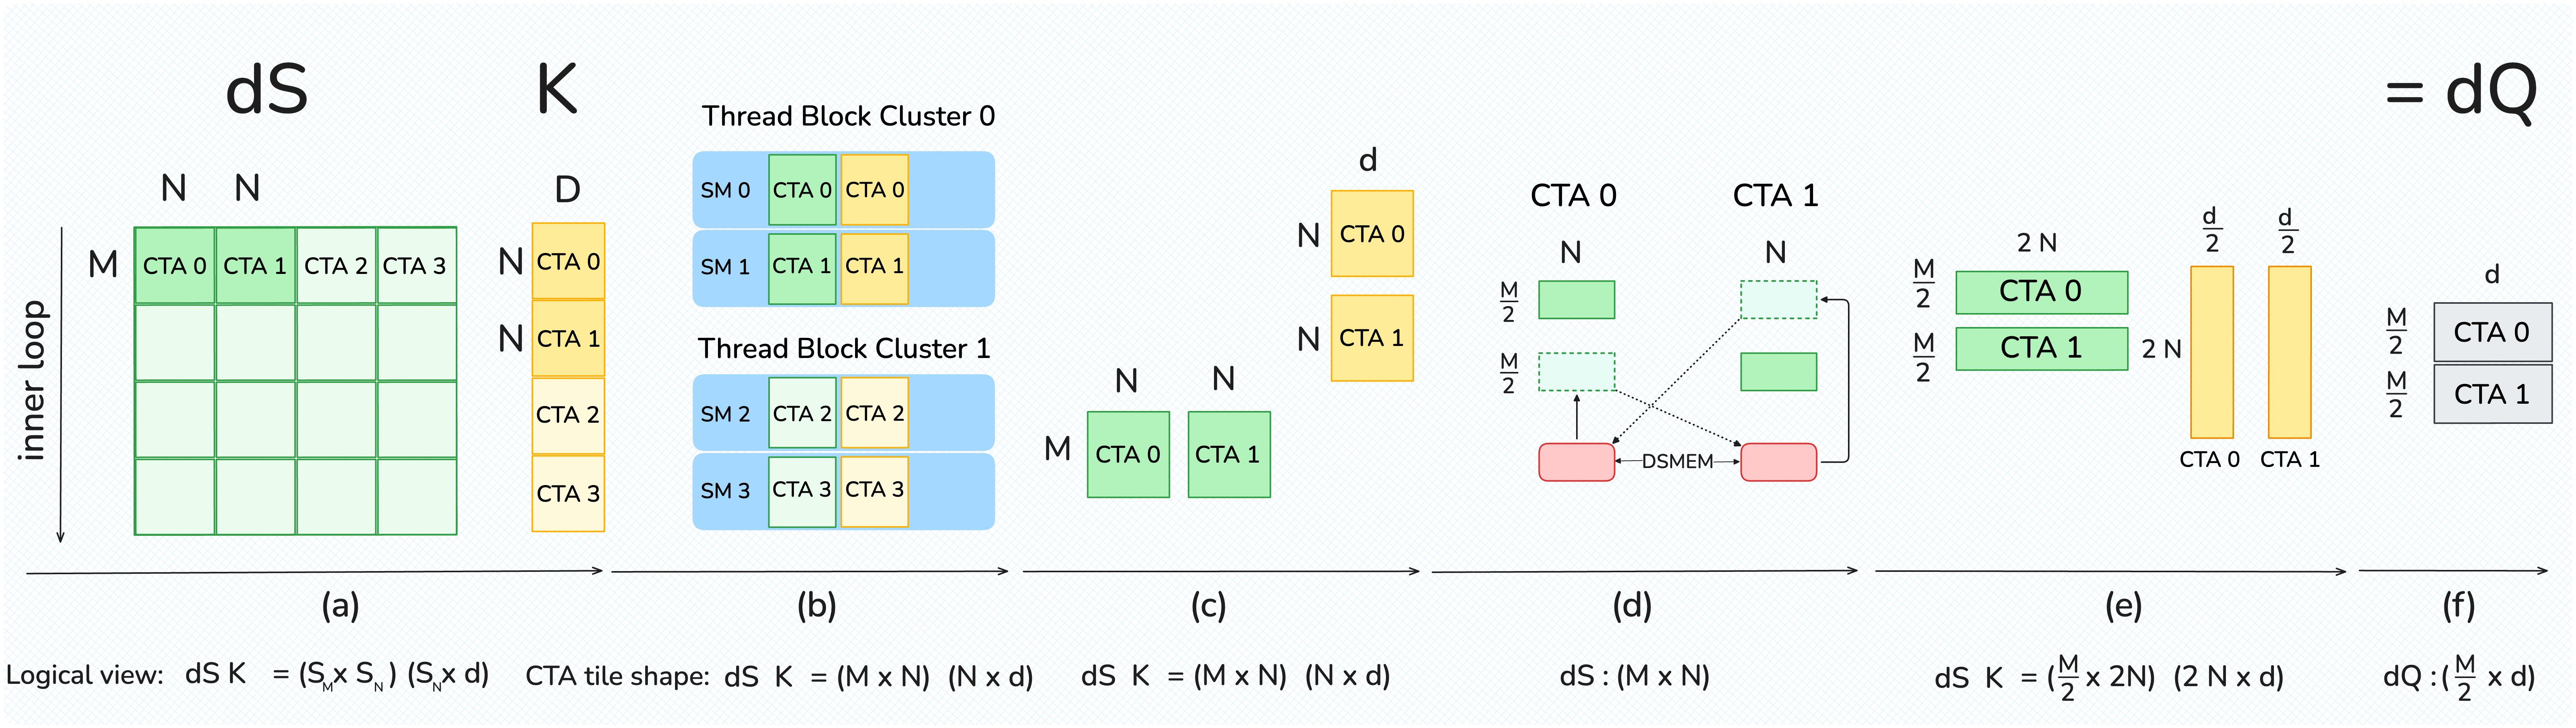
\includegraphics[width=1.0\linewidth]{Figures/2cta_figure.png}
  \caption{在2-CTA后向传播dQ步骤中，CTA对使用DSMEM交换$dS$块的一半，使每个CTA构成$({\frac{M}{2}} \times 2N)$操作数，并可使用翻倍规约运行CTA对UMMA。}
  \label{fig:2cta_figure}
\end{figure*}

\subsubsection{2-CTA后向传播：减少共享内存流量和全局原子加操作}

即使采用改进的流水线且十个GEMM操作数中有两个常驻于张量内存，共享内存带宽仍然主导后向传播。在五个GEMM中，其余八个BF16操作数从共享内存加载以供张量核心使用，这种共享内存流量比张量核心计算多消耗约30\%的周期。为进一步缓解这一瓶颈，我们使用Blackwell引入的2-CTA MMA模式，其中输出累加器在M维度上被划分。MMA分块形状为$M=256$，$N=K=128$，两个CTA充当单个更大的块：每个CTA装载并暂存操作数B的一半，只保留自己的累加器切片。

\textbf{共享内存流量}。后向传播有五个GEMM，我们使用MMA分块形状$M=256$，$N=K=128$，这大约将操作数B的共享内存流量减半。在FlashAttention后向传播中，每个CTA持有固定的KV块（在外层循环中跨$N$个CTA并行化），并在内层循环中流式处理M块。$\vdQ$的累积是外层循环中KV序列方向的规约，但2-CTA MMA只分割输出块，不分割规约轴，而$\vdQ$ MMA的规约维度是$N$，它自然地跨CTA对分割。因此，每个CTA仍需要对其拥有的行进行完整规约。为解决规约轴上的这一冲突，我们使用分布式共享内存（DSMEM）在两个CTA之间交换$\vdS$的一半（它们在同一集群中）。这一方法对$\vdS$进行重新排列，使其沿非规约轴分区，每个CTA拥有其$\frac{M}{2}$行并持有完整的$2N$规约。因此，每个CTA的$\vdQ$ MMA分块形状为$(\frac{M}{2}, 2N)(2N, d)$，在张量内存中累积$(\frac{M}{2}, d)$块。在2-CTA MMA模式中，$\vS$、$\vdP$、$\vdV$和$\vdK$的MMA使用$M=256$的分块运行，而$\vdQ$使用$M=128$但翻倍的规约$2N=256$。我们随后相对于1-CTA变体重新排列了软件流水线以隐藏DSMEM延迟。我们在计算前一块的$\vdQ$之前先计算当前块的$\vdP$。$\vdQ$块足够小，可以与$\vP$一起放入TMEM，重用与$\vS$相同的TMEM区域，因此我们不再像1-CTA模式那样为$\vdP$和$\vdQ$重用同一个TMEM区域。通过这种新的流水线排序，我们可以在计算前一次迭代块的$\vdQ$ MMA时，并行计算当前块的逐元素$\vdS$。图~\ref{fig:2cta_figure}说明了$\vdQ$步骤的分解方式。

\textbf{$\vdQ$原子加操作}。这种$\vdQ$分解的一个互补好处是，全局原子规约次数减半。原子更新引入不确定性且代价高昂，因为它们在内层循环的每次迭代中都会发生。因此，每个CTA只写入$\vdQ$块的一半，与1-CTA版本相比执行的全局原子规约次数减半。

\subsubsection{确定性后向传播}

我们的后向内核由于全局内存的跨CTA规约（对$\vdQ$一般情况，GQA情况下还涉及$\vdK$/$\vdV$）而引入了梯度计算的不确定性。为确保可复现性并简化训练期间的可靠调试，我们还提供了确定性执行模式。我们采用的标准解决方案是使用信号量锁串行化全局规约。具体地，写入公共$\vdQ$块的每个CTA必须按预定义的顺序获取锁，执行规约，然后通过递增信号量计数器释放锁。

这种基于锁的方法影响性能的原因有两个：(1) 发出内存屏障以确保信号量写操作在设备范围内可见（正确的获取-释放语义所需）；(2) 每个CTA等待在公共$\vdQ$块上规约的前序CTA完成时引入停顿。在负载不均衡的情况下，CTA顺序的朴素选择可能严重降低性能。总体上，我们在头和批次维度上进行CTA重排（直至L2缓存容量，参见\cref{sec:algo_other}）以减少停顿。对于因果掩码，我们额外以降序启动KV块，以从对角线开始的升序遍历查询块，并按降序的查询块索引排列$\vdQ$规约。这种"最短处理时间优先"（SPT）调度确保没有CTA在其第一次$\vdQ$写操作时被阻塞。
